% META: DONE.1

\section{Нейросетевые методы анализа трёхмерной геометрии}

В последние годы глубокое обучение произвело революцию в анализе трёхмерных данных. Было разработано множество архитектур нейронных сетей, способных работать с облаками точек, сетками, воксельными представлениями и другими форматами 3D-данных. Данный раздел представляет обзор наиболее значимых архитектур, которые послужили теоретической основой для выбора модели в рамках настоящей работы.

\subsection{Облака точек (PointNet и PointNet++)}

Облака точек являются одним из наиболее естественных представлений трёхмерных данных, получаемых, например, с 3D-сканеров. Однако работа с облаками точек сопряжена с рядом уникальных вызовов для глубоких нейронных сетей: данные являются неупорядоченными, нерегулярными и зашумленными \cite{sarker2024}.

PointNet, предложенная Чарльзом Ци и соавторами в 2017 году, стала первой архитектурой, которая могла напрямую обрабатывать неупорядоченные облака точек для задач классификации и сегментации. Ключевая инновация PointNet заключается в использовании симметричной функции (например, max pooling) для агрегации информации от всех точек, что обеспечивает инвариантность к перестановке точек на входе. PointNet извлекает глобальные признаки из всего облака точек, но её недостатком является ограниченная способность учитывать локальную структуру - сеть «не видит» взаимосвязей между соседними точками.

PointNet++ была разработана для преодоления этого ограничения. Архитектура иерархически применяет PointNet к возрастающим по размеру окрестностям точек, что позволяет сети захватывать как локальные, так и глобальные геометрические паттерны. PointNet++ использует механизмы выборки и группировки для построения иерархических представлений, аналогично тому, как свёрточные сети работают с изображениями.

Сравнительные исследования показывают, что PointNet, PointNet++ и DGCNN предлагают разные подходы к эффективному управлению характеристиками и пространственной структурой облаков точек \cite{kang2024}. Однако облака точек как представление имеют фундаментальное ограничение: они теряют информацию о связности и топологии поверхности, которая критически важна для инженерных задач.

\subsection{Динамические графовые свёртки: DGCNN}

DGCNN (Dynamic Graph CNN), предложенная Вангом и соавторами, решает проблему учёта локальной структуры облаков точек путём построения графа k-ближайших соседей (KNN) для каждого слоя сети. В отличие от статических графов, DGCNN динамически перестраивает граф на каждом слое на основе признаков, извлечённых на предыдущем слое. Это позволяет сети адаптивно захватывать как геометрическую близость в евклидовом пространстве, так и семантическую близость в пространстве признаков. Ключевой операцией DGCNN является слой EdgeConv, который для каждой точки вычисляет признаки на основе её связей с соседями в графе. Это позволяет сети эффективно извлекать локальные геометрические паттерны, такие как рёбра, углы, кривизна. Как отмечается в исследованиях, «DGCNN продемонстрировала высокую производительность сегментации благодаря динамическим графовым свёрточным сетям» \cite{bai2020}.

DGCNN нашла широкое применение в задачах классификации и семантической сегментации облаков точек \cite{hao2022}. Однако, как и PointNet, DGCNN работает с облаками точек, а не с полноценными сетчатыми представлениями. Для задач, где важна топологическая информация о связности граней и рёбер (например, распознавание скруглений и фасок), этого может быть недостаточно.

\subsection{Сеточные представления: MeshCNN}

MeshCNN, предложенная Раной Ханоцкой и соавторами на конференции SIGGRAPH 2019, представляет собой принципиально иной подход: сеть работает непосредственно с треугольными сетками, сохраняя топологию поверхности \cite{meshcnn2019}. Это особенно важно для инженерных CAD-задач, где геометрия изначально задаётся в виде B-Rep (грани, рёбра, вершины), а STL-сетка является лишь аппроксимацией, сохраняющей эту топологию.

Основные инновации MeshCNN включают:

\begin{itemize}
    \item Свёртка на рёбрах. В отличие от традиционных свёрточных сетей, работающих с регулярными сетками (пикселями), MeshCNN определяет свёртку на рёбрах треугольной сетки. Каждое ребро связано с четырьмя треугольниками (по два с каждой стороны) и, соответственно, с четырьмя соседними рёбрами. Эта топологическая окрестность служит «рецептивным полем» для свёртки \cite{meshcnn2019}.
    \item Пулинг на сетке. MeshCNN включает механизм пулинга (объединения), который уменьшает разрешение сетки путём коллапса рёбер (edge collapse). При этом сеть обучается выбирать, какие рёбра «наименее информативны» для текущей задачи и могут быть объединены (важно, что пулинг обратим - предусмотрен слой анпулинга (unpooling) для восстановления исходной топологии для сегментации).
    \item Инвариантность к изотропной триангуляции. Одной из ключевых особенностей MeshCNN является устойчивость к разным способам триангуляции одной и той же геометрии. Сеть использует инвариантные признаки (углы между гранями, отношения площадей, синусы двугранных углов), которые не зависят от того, как именно поверхность разбита на треугольники. В исходной публикации MeshCNN была продемонстрирована на задачах классификации 3D-форм (датасет SHREC) и семантической сегментации (сегментация человеческих фигур на части) \cite{meshcnn2019}.
\end{itemize}

Краткая конструкция отображена на рис.~\ref{fig:meshcnn-arch}

\begin{figure}[h]
    \centering
    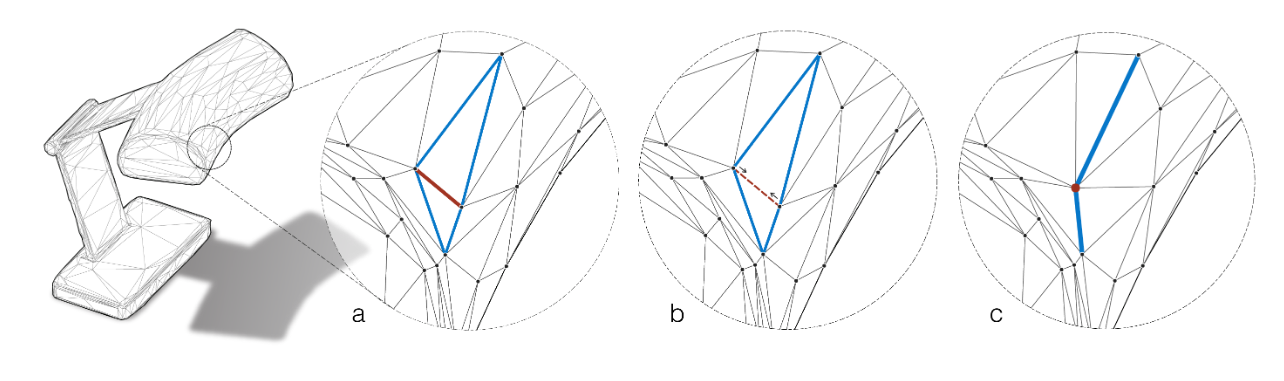
\includegraphics[width=0.8\linewidth]{figures/meshcnn_arch.png}
    \caption{Основной шаг MeshCNN \cite{meshcnn2019}}
    \label{fig:meshcnn-arch}
\end{figure}

Для задачи сегментации CAD-моделей по типам порождающих операций MeshCNN обладает рядом важных преимуществ:
\begin{itemize}
\item сохраняет топологию сетки, что важно для распознавания рёбер, граней и их взаимосвязей;
\item оперирует инвариантными признаками, что снижает чувствительность к конкретному способу триангуляции;
\item позволяет выполнять классификацию и сегментацию в едином фреймворке;
\item имеет открытую реализацию, доступную для адаптации под специфические задачи.
\end{itemize}

Именно эти свойства послужили основой для выбора MeshCNN в качестве базовой архитектуры нейросетевого контура в настоящей работе.

\subsection{Сравнительный анализ архитектур для задачи сегментации CAD-операций}

\begin{table}[h]
\centering
\begin{tabular}{|p{3.5cm}|p{2.5cm}|p{2.5cm}|p{2.5cm}|p{2.5cm}|}
\hline
Характеристика & PointNet & PointNet++ & DGCNN & MeshCNN \\
\hline
Входное представление & Облако точек & Облако точек & Облако точек & Треугольная сетка \\
\hline
Учёт локальной структуры & Только глобальная & Иерархический & Граф k-NN & Топологическая окрестность ребра \\
\hline
Инвариантность к перестановке & Да (max pooling) & Да & Да (симметричная агрегация) & Да (свёртка на рёбрах) \\
\hline
Сохранение топологии & Нет & Нет & Частично (через граф) & Да \\
\hline
Пригодность для распознавания рёбер & Низкая & Средняя & Средняя & Высокая \\
\hline
Вычислительная сложность & Низкая & Средняя & Средняя & Высокая (из-за динамической топологии) \\
\hline
\end{tabular}
\end{table}

Как следует из таблицы, MeshCNN является наиболее подходящей архитектурой для задачи сегментации CAD-моделей по типам операций, поскольку она сохраняет топологическую информацию о рёбрах и гранях, критически важную для распознавания инженерной семантики.

